\documentclass{standalone}
\usepackage{tikz}
\usetikzlibrary{patterns, positioning}


\begin{document}
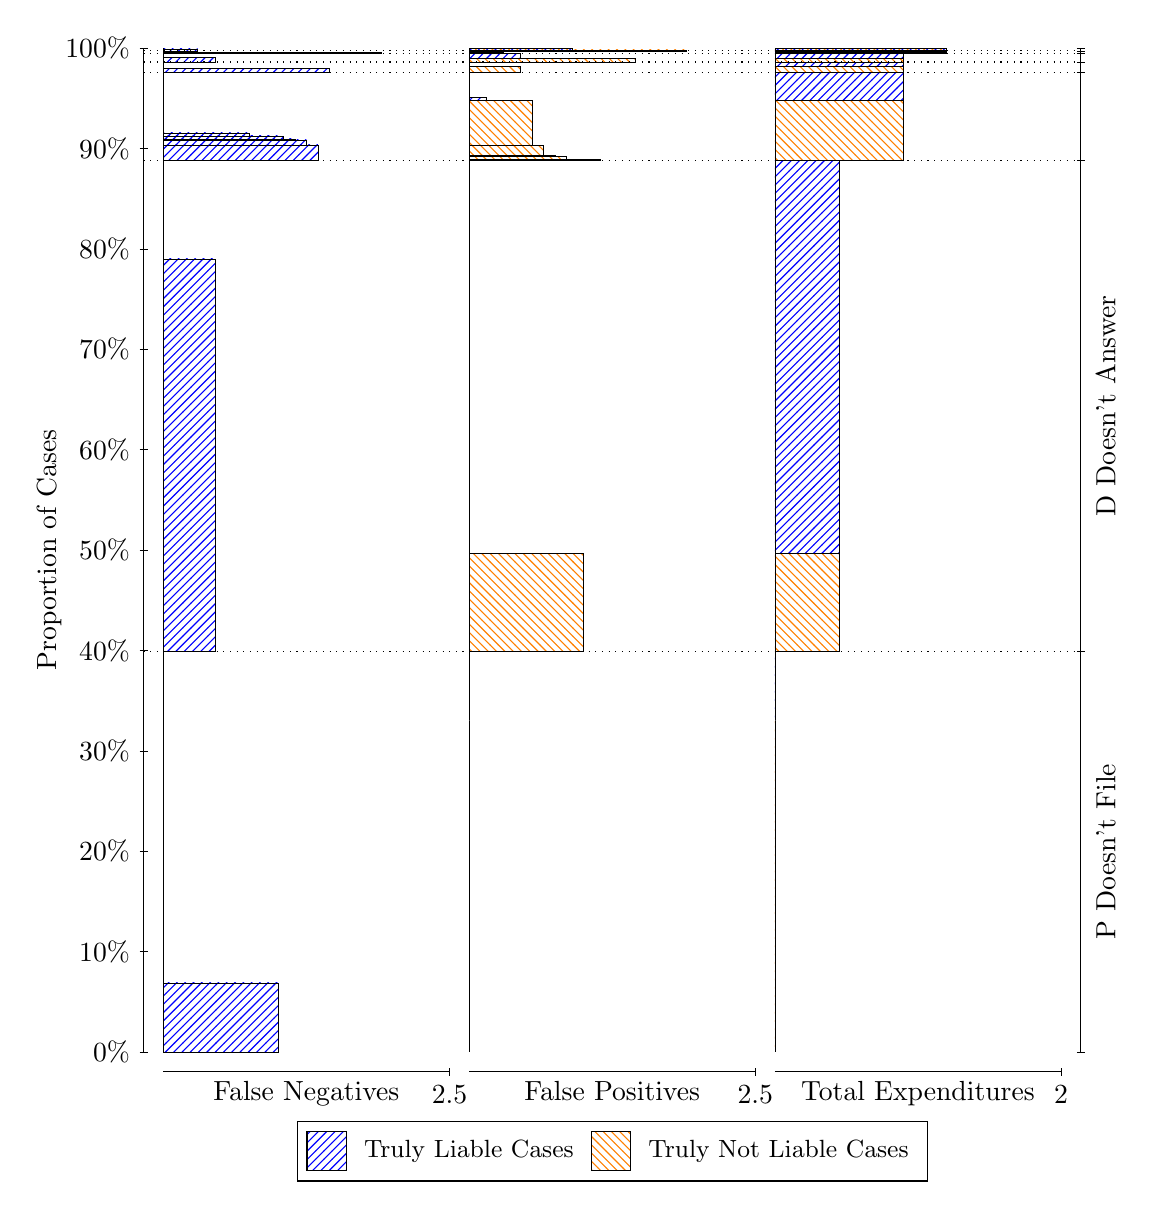
\begin{tikzpicture}
\draw[black, very thin] (1.5,1.75) -- (1.5,14.5);
\node[rotate=90, text=black, anchor=center] at (0.3, 8.125) {Proportion of Cases};
\draw[black, very thin] (1.45,1.75) -- (1.55,1.75);
\node[text=black, anchor=east] at (1.45, 1.75) {0\%};
\draw[black, very thin] (1.45,3.025) -- (1.55,3.025);
\node[text=black, anchor=east] at (1.45, 3.025) {10\%};
\draw[black, very thin] (1.45,4.3) -- (1.55,4.3);
\node[text=black, anchor=east] at (1.45, 4.3) {20\%};
\draw[black, very thin] (1.45,5.575) -- (1.55,5.575);
\node[text=black, anchor=east] at (1.45, 5.575) {30\%};
\draw[black, very thin] (1.45,6.85) -- (1.55,6.85);
\node[text=black, anchor=east] at (1.45, 6.85) {40\%};
\draw[black, very thin] (1.45,8.125) -- (1.55,8.125);
\node[text=black, anchor=east] at (1.45, 8.125) {50\%};
\draw[black, very thin] (1.45,9.4) -- (1.55,9.4);
\node[text=black, anchor=east] at (1.45, 9.4) {60\%};
\draw[black, very thin] (1.45,10.675) -- (1.55,10.675);
\node[text=black, anchor=east] at (1.45, 10.675) {70\%};
\draw[black, very thin] (1.45,11.95) -- (1.55,11.95);
\node[text=black, anchor=east] at (1.45, 11.95) {80\%};
\draw[black, very thin] (1.45,13.225) -- (1.55,13.225);
\node[text=black, anchor=east] at (1.45, 13.225) {90\%};
\draw[black, very thin] (1.45,14.5) -- (1.55,14.5);
\node[text=black, anchor=east] at (1.45, 14.5) {100\%};

\draw[black, very thin] (13.4,1.75) -- (13.4,14.5);
\draw[black, very thin] (13.35,1.75) -- (13.45,1.75);
\node[anchor=west] at (13.35, 1.75) {};
\draw[black, very thin] (13.35,6.8357) -- (13.45,6.8357);
\node[anchor=west] at (13.35, 6.8357) {};
\draw[black, very thin] (13.35,13.07) -- (13.45,13.07);
\node[anchor=west] at (13.35, 13.07) {};
\draw[black, very thin] (13.35,14.186) -- (13.45,14.186);
\node[anchor=west] at (13.35, 14.186) {};
\draw[black, very thin] (13.35,14.322) -- (13.45,14.322);
\node[anchor=west] at (13.35, 14.322) {};
\draw[black, very thin] (13.35,14.432) -- (13.45,14.432);
\node[anchor=west] at (13.35, 14.432) {};
\draw[black, very thin] (13.35,14.463) -- (13.45,14.463);
\node[anchor=west] at (13.35, 14.463) {};
\draw[black, very thin] (13.35,14.5) -- (13.45,14.5);
\node[anchor=west] at (13.35, 14.5) {};

\draw[black, very thin, pattern color=blue, pattern=north east lines] (1.75,1.75) rectangle (3.2033,2.6271);
\draw[black, very thin, pattern color=orange, pattern=north west lines] (1.75,2.6271) rectangle (1.75,6.8357);
\draw[black, very thin, pattern color=blue, pattern=north east lines] (1.75,6.8357) rectangle (2.404,11.823);
\draw[black, very thin, pattern color=orange, pattern=north west lines] (1.75,11.823) rectangle (1.75,13.07);
\draw[black, very thin, pattern color=blue, pattern=north east lines] (1.75,13.07) rectangle (3.712,13.271);
\draw[black, very thin, pattern color=blue, pattern=north east lines] (1.75,13.271) rectangle (3.5667,13.332);
\draw[black, very thin, pattern color=blue, pattern=north east lines] (1.75,13.332) rectangle (3.4213,13.347);
\draw[black, very thin, pattern color=blue, pattern=north east lines] (1.75,13.347) rectangle (3.276,13.384);
\draw[black, very thin, pattern color=blue, pattern=north east lines] (1.75,13.384) rectangle (3.1307,13.385);
\draw[black, very thin, pattern color=blue, pattern=north east lines] (1.75,13.385) rectangle (2.84,13.422);
\draw[black, very thin, pattern color=orange, pattern=north west lines] (1.75,13.422) rectangle (1.75,14.186);
\draw[black, very thin, pattern color=blue, pattern=north east lines] (1.75,14.186) rectangle (3.8573,14.244);
\draw[black, very thin, pattern color=orange, pattern=north west lines] (1.75,14.244) rectangle (1.75,14.322);
\draw[black, very thin, pattern color=blue, pattern=north east lines] (1.75,14.322) rectangle (2.404,14.386);
\draw[black, very thin, pattern color=orange, pattern=north west lines] (1.75,14.386) rectangle (1.75,14.432);
\draw[black, very thin, pattern color=blue, pattern=north east lines] (1.75,14.432) rectangle (4.5113,14.444);
\draw[black, very thin, pattern color=orange, pattern=north west lines] (1.75,14.444) rectangle (1.75,14.463);
\draw[black, very thin, pattern color=blue, pattern=north east lines] (1.75,14.463) rectangle (2.186,14.489);
\draw[black, very thin, pattern color=orange, pattern=north west lines] (1.75,14.489) rectangle (1.75,14.5);
\draw[black, very thin, pattern color=orange, pattern=north west lines] (5.6333,1.75) rectangle (5.6333,5.9585);
\draw[black, very thin, pattern color=blue, pattern=north east lines] (5.6333,5.9585) rectangle (5.6333,6.8357);
\draw[black, very thin, pattern color=orange, pattern=north west lines] (5.6333,6.8357) rectangle (7.0867,8.0829);
\draw[black, very thin, pattern color=blue, pattern=north east lines] (5.6333,8.0829) rectangle (5.6333,13.07);
\draw[black, very thin, pattern color=orange, pattern=north west lines] (5.6333,13.07) rectangle (7.3047,13.083);
\draw[black, very thin, pattern color=orange, pattern=north west lines] (5.6333,13.083) rectangle (7.014,13.084);
\draw[black, very thin, pattern color=orange, pattern=north west lines] (5.6333,13.084) rectangle (6.8687,13.121);
\draw[black, very thin, pattern color=orange, pattern=north west lines] (5.6333,13.121) rectangle (6.7233,13.137);
\draw[black, very thin, pattern color=orange, pattern=north west lines] (5.6333,13.137) rectangle (6.578,13.268);
\draw[black, very thin, pattern color=orange, pattern=north west lines] (5.6333,13.268) rectangle (6.4327,13.834);
\draw[black, very thin, pattern color=blue, pattern=north east lines] (5.6333,13.834) rectangle (5.8513,13.871);
\draw[black, very thin, pattern color=blue, pattern=north east lines] (5.6333,13.871) rectangle (5.6333,14.186);
\draw[black, very thin, pattern color=orange, pattern=north west lines] (5.6333,14.186) rectangle (6.2873,14.264);
\draw[black, very thin, pattern color=blue, pattern=north east lines] (5.6333,14.264) rectangle (5.6333,14.322);
\draw[black, very thin, pattern color=orange, pattern=north west lines] (5.6333,14.322) rectangle (7.7407,14.367);
\draw[black, very thin, pattern color=blue, pattern=north east lines] (5.6333,14.367) rectangle (6.2873,14.432);
\draw[black, very thin, pattern color=orange, pattern=north west lines] (5.6333,14.432) rectangle (6.0693,14.452);
\draw[black, very thin, pattern color=blue, pattern=north east lines] (5.6333,14.452) rectangle (5.6333,14.463);
\draw[black, very thin, pattern color=orange, pattern=north west lines] (5.6333,14.463) rectangle (8.3947,14.475);
\draw[black, very thin, pattern color=blue, pattern=north east lines] (5.6333,14.475) rectangle (6.9413,14.5);
\draw[black, very thin, pattern color=orange, pattern=north west lines] (9.5167,1.75) rectangle (9.5167,5.9585);
\draw[black, very thin, pattern color=blue, pattern=north east lines] (9.5167,5.9585) rectangle (9.5167,6.8357);
\draw[black, very thin, pattern color=orange, pattern=north west lines] (9.5167,6.8357) rectangle (10.334,8.0829);
\draw[black, very thin, pattern color=blue, pattern=north east lines] (9.5167,8.0829) rectangle (10.334,13.07);
\draw[black, very thin, pattern color=orange, pattern=north west lines] (9.5167,13.07) rectangle (11.152,13.834);
\draw[black, very thin, pattern color=blue, pattern=north east lines] (9.5167,13.834) rectangle (11.152,14.186);
\draw[black, very thin, pattern color=orange, pattern=north west lines] (9.5167,14.186) rectangle (11.152,14.264);
\draw[black, very thin, pattern color=blue, pattern=north east lines] (9.5167,14.264) rectangle (11.152,14.322);
\draw[black, very thin, pattern color=orange, pattern=north west lines] (9.5167,14.322) rectangle (11.152,14.367);
\draw[black, very thin, pattern color=blue, pattern=north east lines] (9.5167,14.367) rectangle (11.152,14.432);
\draw[black, very thin, pattern color=orange, pattern=north west lines] (9.5167,14.432) rectangle (11.697,14.452);
\draw[black, very thin, pattern color=blue, pattern=north east lines] (9.5167,14.452) rectangle (11.697,14.463);
\draw[black, very thin, pattern color=orange, pattern=north west lines] (9.5167,14.463) rectangle (11.697,14.475);
\draw[black, very thin, pattern color=blue, pattern=north east lines] (9.5167,14.475) rectangle (11.697,14.5);
\draw[black, dotted] (1.5,6.8357) -- (13.4,6.8357);
\draw[black, dotted] (1.5,13.07) -- (13.4,13.07);
\draw[black, dotted] (1.5,14.186) -- (13.4,14.186);
\draw[black, dotted] (1.5,14.322) -- (13.4,14.322);
\draw[black, dotted] (1.5,14.432) -- (13.4,14.432);
\draw[black, dotted] (1.5,14.463) -- (13.4,14.463);
\draw[black, very thin] (1.75,1.5) -- (5.3833,1.5);
\node[text=black, anchor=north] at (3.5667, 1.5) {False Negatives};
\draw[black, very thin] (5.3833,1.45) -- (5.3833,1.55);
\node[text=black, anchor=north] at (5.3833, 1.45) {2.5};

\draw[black, very thin] (5.6333,1.5) -- (9.2667,1.5);
\node[text=black, anchor=north] at (7.45, 1.5) {False Positives};
\draw[black, very thin] (9.2667,1.45) -- (9.2667,1.55);
\node[text=black, anchor=north] at (9.2667, 1.45) {2.5};

\draw[black, very thin] (9.5167,1.5) -- (13.15,1.5);
\node[text=black, anchor=north] at (11.333, 1.5) {Total Expenditures};
\draw[black, very thin] (13.15,1.45) -- (13.15,1.55);
\node[text=black, anchor=north] at (13.15, 1.45) {2};

\node[text=black, centered, rotate=90] at (13.72, 4.2928) {P Doesn't File};
\node[text=black, centered, rotate=90] at (13.72, 9.9528) {D Doesn't Answer};






\draw (7.449999999999999,1.5) node[draw=none] (baseCoordinate) {};
\begin{scope}[align=center]
        \matrix[scale=0.5, draw=black, below=0.5cm of baseCoordinate, nodes={draw}, column sep=0.1cm]{
            \node[rectangle, draw, minimum width=0.5cm, minimum height=0.5cm, pattern color=blue, pattern=north east lines] {}; &
            \node[draw=none, font=\small, text=black] (B) {Truly Liable Cases}; &
            \node[rectangle, draw, minimum width=0.5cm, minimum height=0.5cm, pattern color=orange, pattern=north west lines] {}; &
            \node[draw=none, font=\small, text=black] (B) {Truly Not Liable Cases}; \\
            };
\end{scope}

\end{tikzpicture}
\end{document}